%\RequirePackage{snapshot}
\documentclass[10pt,a4paper]{article}
%\RequirePackage{graphics}
\usepackage[dvips]{graphics}
\RequirePackage{lineno} 
\usepackage[pdftex]{color, graphicx}
\usepackage{amsmath, amsthm}
%\usepackage{amssymb}
\usepackage{multirow}
\usepackage{subfigure}
\usepackage{xspace}
\usepackage{cite}
\usepackage{ifthen}

\RequirePackage{lineno}
\setlength{\oddsidemargin}{0cm}
\setlength{\textwidth}{16cm}
\setlength{\topmargin}{-15mm}
\setlength{\textheight}{245mm}
\usepackage[pdfauthor={MT2 Team},bookmarks=true]{hyperref} % bookmarks

%\title{\huge{Charge and flavour ratios in SUSY leptonic final states} \\
\title{\huge{  
Data Delivery Architecture for CMS Level-1 Tracking Trigger} \\
\ \  \\
\large{ }}
\author{our names}
\vspace{2cm}
\date{\today}

%========================================================================

%\usepackage{topcapt}
%\input{svjour.cls}
%\input{cms-tdr-note.cls}
%\input{cms-tdr.cls}
\usepackage{hepparticles}
\usepackage{heppennames2}
\usepackage{ptdr-definitions}
%\usepackage{pennames-ital}

\newcommand{\MT}{\ensuremath{M_{\mathrm{T}}}\xspace}
\newcommand{\MTmax}{\ensuremath{\MT^{\mathrm{max}}}\xspace}
\newcommand{\MTmin}{\ensuremath{\MT^{\mathrm{min}}}\xspace}
\newcommand{\SSee}{\ensuremath{\Pepm\Pepm}\xspace}
\newcommand{\SSem}{\ensuremath{\Pepm\PGmpm}\xspace}
\newcommand{\SSmm}{\ensuremath{\PGmpm\PGmpm}\xspace}
\newcommand{\threel}{3\ensuremath{\ell}\xspace}
\newcommand{\Mll}{\ensuremath{M_{\ell\ell}}\xspace}
\newcommand{\MSFOS}{\ensuremath{M_{\mathrm{SFOS}}}\xspace}
\newcommand{\ptlll}{\ensuremath{\pt(\ell\ell\ell)}\xspace}
\newcommand{\ptlllvec}{\ensuremath{\ptvec(\ell\ell\ell)}\xspace}
\newcommand{\ptveclll}{\ensuremath{\ptvec(\ell\ell\ell)}\xspace}
\newcommand{\DPhilllMET}{\ensuremath{\Delta\phi\left(\ptlllvec,\ptvecmiss\right)}\xspace}
\newcommand{\Mlll}{\ensuremath{M_{\ell\ell\ell}}\xspace}
\newcommand{\Mjj}{\ensuremath{M_{\mathrm{jj}}}\xspace}
\newcommand{\theLumi}{\ensuremath{35.9\fbinv}\xspace}
\newcommand{\WHtoWWW}{\ensuremath{\cmsSymbolFace{WH}\to\cmsSymbolFace{WWW}^{(*)}}\xspace}
\newcommand{\Wmp}{\PWmp}
%\newcommand{\Pemp}{\ensuremath{\cmsSymbolFace{e}^{\mp}}\xspace}
\newcommand{\WWW}{\ensuremath{\Wpm\Wpm\Wmp}\xspace}
\newcommand{\SSWW}{\ensuremath{\Wpm\Wpm}\xspace}%use this to avoid useless space between the Wpm
\newcommand{\ttW}{\ensuremath{\ttbar\Wpm}\xspace}%use this to avoid useless space between the Wpm
\newcommand{\ttZ}{\ensuremath{\ttbar\PZ}\xspace}%use this to avoid useless space between the Wpm
\newcommand{\ttV}{\ensuremath{\ttbar\mathrm{V}}\xspace}%use this to avoid useless space between the Wpm
\newcommand{\ttH}{\ensuremath{\ttbar\mathrm{H}}\xspace}%use this to avoid useless space between the Wpm
\newcommand{\eTL}{\ensuremath{\epsilon_{\mathrm{TL}}}\xspace}
\newcommand{\etl}{\eTL}
\newcommand{\ptl}{\ensuremath{\pt^{\ell}}\xspace}
\newcommand{\ptvecl}{\ensuremath{\ptvec^{\,\ell}}\xspace}
\newcommand{\ptlvec}{\ptvecl}
\newcommand{\ptjet}{\ensuremath{\pt^{\text{jet}}}\xspace}
\newcommand{\ptvecjet}{\ensuremath{\ptvec^{\,\text{jet}}}\xspace}
\newcommand{\ptjetvec}{\ptvecjet}
\newcommand{\ptcor}{\ensuremath{\pt^{\text{corr}}}\xspace}

\begin{document}

\hyphenation{had-ron-i-za-tion}
\hyphenation{cal-or-i-me-ter}
\hyphenation{de-vices}
%\input{newcommand}




\maketitle

\begin{abstract}
\end{abstract}

\newpage
%
\tableofcontents
\linenumbers
\newpage

%%%%%%%% Definitions
%\def\eslash{{\hbox{$E$\kern-0.5em\lower-.05ex\hbox{/}\kern-0.10em}}}
%\def\MET{\mbox{$\eslash_T$}}
%\def\hslash{{\hbox{$H$\kern-0.5em\lower-.05ex\hbox{/}\kern-0.10em}}}
%\def\MHT{\mbox{$\hslash_T$\ }}
%%%%%%%%%%%%%%%%%%%%%%%%%%%%%%%%  Begin text %%%%%%%%%%%%%%%%%%%%%%%%%%%%%


\section{Introduction \label{sec:intro}}

\subsection{Motivation}


In order to maximize the potential for the discovery, CMS must preserve or improve its ability to identify, in real time, events with signatures consistent with the Higgs boson and new particle decays for high luminosity LHC (HL-LHC) operation. This is a highly non-trivial task given the high pile-up conditions anticipated in the HL-LHC era. At LHC, the only major detector not used at L1 trigger are the silicon tracking detectors. It has become clear that the development of the L1 tracking trigger system is of utmost importance for CMS for the HL-LHC, in order to maintain physics acceptances for basic objects (leptons, photons, jets and MET).  Without L1 tracking, most quantities traditionally used for L1 are washed out and become unusable due to the huge "background" created by the overlap of too many collisions in the same beam crossing. This would put most of the anticipated physics program out of reach. 

Consequently, the design of the Phase-II CMS Tracker must allow for an effective implementation of the tracking trigger.... (add a few sentences here).  Because the construction of the Phase-II Tracker will take many years, its tracker design must be finalized sooner.    Silicon-based Level-2 tracking trigger systems based on associative memory were successfully implemented in the past~\cite{bib:Rist-89}~\cite{bib:Ade-06}~\cite{bib:Ade-07} and are being actively explored at present~\cite{bib:FTK-TP}~\cite{bib:FTK-TDR}. Experience with these systems will serve as useful input to the design of the CMS L1 tracking trigger. However the higher occupancies anticipated at the HL-LHC and the low latencies required at L1 (about 10~$\mu$s total and a few $\mu$s for the track finding stage) present us with a formidable set of challenges that we need to attack with a well organized R\&D campaign in order to be successful. A silicon-based L1 tracking trigger has never been realized at this scale and thus it is imperative that its feasibility be demonstrated before the design of the Phase-II Tracker can be finalized. To achieve this goal, a Vertical Slice System Demonstration system has been designed and built, using the assocative memory approach, and the  system comprises a full tracking trigger path and uses simulated high-luminosity data to measure trigger latency and efficiency, to study overall system performance and to identify appropriate solutions to possible bottlenecks. The demonstration system is by no means meant to be final  but serves the purpose of an existence proof.

\subsection{Associative Memory approach}

The Associative Memory solves the combinatorial problem, inherent to this kind of pattern recognition algorithms, by employing a massively parallel architecture to compare each detector hit to a large number of pre-calculated geometrical patterns simultaneously. Then, the selected patterns or roads are processed using fast FPGAs to perform track fitting. Since each pattern corresponds to a very narrow "road" through the detector, the usual helical fit is much simplified and fast by using a pre-calculated set of parameter values for the center of the road and applying corrections that are a linear function of the actual hit positions in each layer.  Because roads are narrow, this linear approximation works very well and the track fitting stage is much simplified and fast~\cite{bib:Ann-09} using pre-calculated track parameters for hits in the center of the road, and applying corrections that are linear in the exact position of the hits in each layer. Although roads are narrow, there is still a finite probability that multiple hits may fall within the same road for a given detector layer, requiring multiple fits with different hit combinations and leading to longer execution times. To reduce latency, the probability of occurrence of multiple hits in the same road must be made as small as possible by making the roads as narrow as possible and, consequently, increasing the total number of them we need to store in the AM to cover the parameter space of interest. This is why an aggressive R\&D program focused on achieving higher AM densities is an important component of the effort needed to reach the unprecedented low latencies required for silicon based tracking at the HL-LHC crossing frequency.

As soon as all the hits have been stored in the AM, found tracks are ready to be output. The whole latency incurred is the time needed to load the hits plus the time to read the matched patterns. In this sense the AM is hard to beat for this particular task. However, the design of an Associative Memory system capable of dealing with the much higher complexity of the HL-LHC collisions, and with the much shorter latency required by Level 1 triggering, poses significant, still unsolved, technical challenges. While we have a very aggressive R\&D program at Fermilab to advance the state-of-the-art associative memory technology (the 3D VIPRAM~\cite{bib:VIP-11} R\&D), we are open to possible new alternative approaches. Since the Associative Memory approach is a proven solution to tracking triggers in a hadron collider environment, it is chosen as the baseline for this demonsttration. 



\noindent 



%Main components

%Fiber data transmission,
%ATCA crates,
%Full mesh backplane,
%Fiber receivers,
%Pattern Recognition Boards,
%Pattern Recognition Mezzanines,
%AM as a possible incarnation (3d technology),
%Inter-tower communication,

%Bandwidth and latency considerations


\clearpage
\section{CMS Track Trigger\label{sec:tracktrigger}}
\section{System Demonstration Hardware Setup \label{sec:hardwaresetup}}


(we have more existing materials for this section, to be included soon).

The demonstration system comprises a full trigger path using a single tracking trigger tower (1/48 of the full detector). It uses simulated high-luminosity data as input to measure trigger latency and efficiency, to study overall system performance, and to identify appropriate solutions to possible bottlenecks. 
The demonstration system achieved excellent performance in terms of tracking efficiency and momentum resolution within a very short latency (2.5 microseconds). This latency includes the time needed for data delivery to the trigger towers, for pattern recognition, and for track fitting. This demonstration is proof that fast data delivery, fast pattern recognition, and track fitting can be implemented successfully using the full mesh ATCA architecture and an associative memory approach. While the focus here is on the HL-LHC, the techniques developed are rather generic and could have other applications beyond tracking triggers, within and outside HEP.

The Fermilab/LPC vertical-slice system demonstration is based on Pulsar 2b boards arranged in two ATCA shelves as shown in Figure n. The Pulsar2b is a custom ATCA full mesh enabled FPGA-based processor board which has been designed with the goal of creating a scalable architecture abundant in flexible, non-blocking, high bandwidth interconnections. The full mesh backplane interconnections effectively blur the distinction between FPGAs, and allow options for data sharing in both space and time..... add a few more sentences references here. 

Twelve Pulsar2b boards in the lower shelf function as Data Source Boards, with another twelve Pulsar 2b boards in the upper shelf functioning as the Pattern Recognition Boards.  Connecting the two shelves are 120 QSFP+ active optical cables, each with 4 bidirectional lanes each running at 10Gbps, for a total capacity of 4.8Tbps in each direction. All Pulsar2b boards in the system are synchronized to a common master clock optical link. This clock is provided by a CERN TTCcx board that encodes a simulated 40MHz bunch crossing clock and several control signals. The optical link is received by one Pulsar2b board on each shelf.  From this Pulsar2b board the master clock and other control bits are distributed to other Pulsar2b boards in the shelf over dedicated clock lines  on the ATCA backplane. 

Simulated event data are first loaded into the Data Source Board FPGAs and then, when triggered by bunch crossing signal, are transmitted over the 120 QSFP+ optical links at full speed to the Pattern Recognition Boards in the upper shelf.  These 12 Pattern Recognition Boards receive the incoming data, perform sophisticated time multiplexed data transfers over the full mesh ATCA backplane, and finally present the event data to the FMC mezzanine cards (Figure 2).  The pattern matching and track fitting algorithms for a given event are implemented on one FMC mezzanine card. Each mezzanine card uses a pair of Xilinx Kintex UltraScale FPGAs, the master FPGA performs track finding functions while the slave FPGA is used to emulate associative memory functionalities with a subset of AM pattern banks. Emulation of the AM functions in a fast, modern FPGA enables us to quickly evaluate and optimize the performance of the AM-FPGA interface and internal AM logic features.




\subsection{Vertical Slice Demonstrator System: Overview and Methodology}

\noindent The flexible architecture described above lends itself to an early technical demonstration of the system. The main goal of the demonstration system is to identify possible problems in the architecture design and, hopefully, find solutions. We can study, measure and optimize trigger latency and efficiencies at different stages of the system using hardware prototypes developed. This involves extensive simulation work, to guide the hardware implementation and to compare actual measurements with expectations. The Vertical Slice Demonstration System is shown in Figure~\ref{fig:VS_TBench}. Each stage is described in more detail in the following sections. 

Although the architecture is flexible enough to allow for different configurations, for the demonstration, we will use the specific configuration with ten Pattern Recognition Boards as an example. This demo system has been implemented in stages, at mezzanine level, board level, crate level. These different stages would naturally proceed in sequence, from the bottom up. This way, we have the opportunity to learn along the way about the performance of the different components of the system before having to decide exactly how the whole thing will be cabled up. Also, the extra crate, with three neighbor towers, needs to come into play only at a very advanced stage, towards the end when the core system dynamics has been demonstrated. In fact, for proof-of-principle demonstration, the extra crate with three neigbhor towers are not needed once the core system performance is understood. 

\begin{figure}[ht!]
\centering
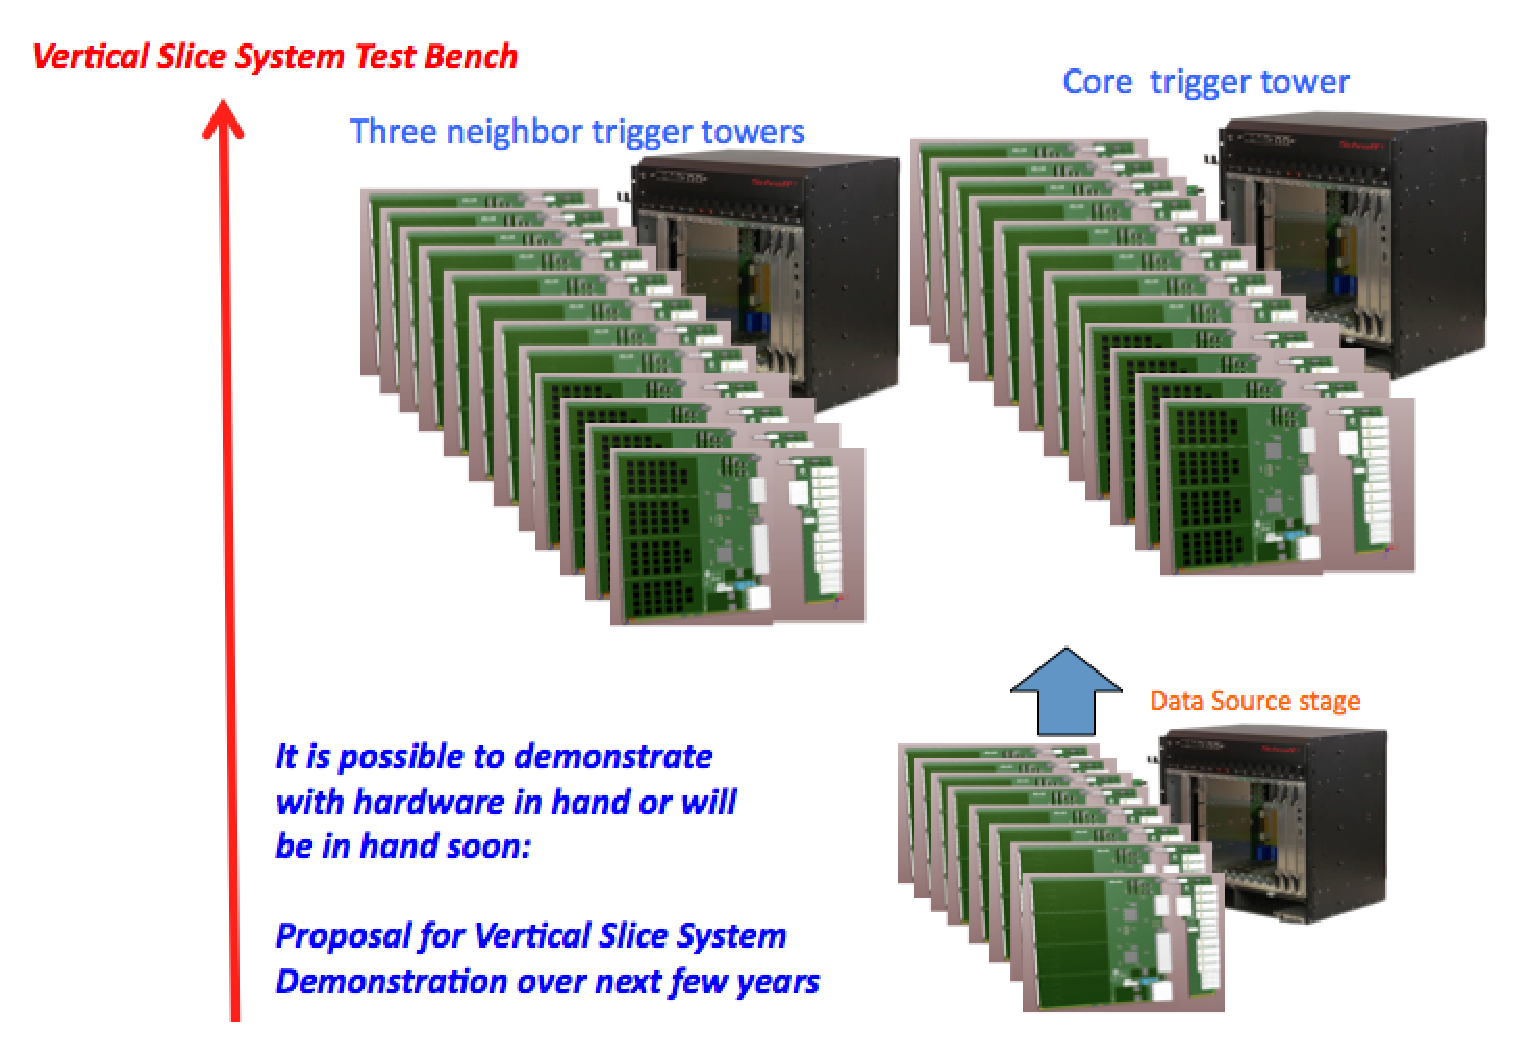
\includegraphics[width=0.8\columnwidth]{Plots/VSTBench.eps}
\caption{Vertical slice test bench principle.}
\label{fig:VS_TBench}
\end{figure}

\subsubsection{Data Source Stage}

\noindent The Data Source mimics the data flow out of the upgraded Phase II outer-tracker running at the HL-LHC. It will drive 300+ fibers (one/module) to the trigger tower under study exactly as the data were coming from the real detector at high luminosity and full speed. Each fiber connection will transmit data at 3.25~Gbps payload bandwidth, in the same way as the actual modules in the future real system. The data will be derived from simulation, appropriately formatted, stored into on-board memories, and then played back at full speed.  The Pulsar IIb board can be used for Data Source stage. 

\subsubsection{Data Input}

\noindent The Data Input Blade (DIB) is responsible for receiving data from the upstream detector electronics (or Data Source output) and transferring them to the PRBs. Up to about 40 fiber links will be received by each DIB. These input links may terminate on the RTM or mezzanine cards. Input fiber links are nominally 3.25~Gb/s payload bandwidth. Again, the Pulsar IIb board can be used as DIB. The Data Input Board will perform zero suppression, pack the stubs into a new format and send them to the PRBs. Current estimates indicate that a rate of about 200 stubs per event per trigger tower, which yields a data rate of roughly 256~Gb/s (200 stubs*32~bits/25~ns) entering each trigger tower on average.

\noindent As an example, in the configuration with eight DIBs and four PRBs, each DIB will be receiving an average of about 256/8 = 32 Gb/s of stub data (after zero suppression). Each of the eight DIBs in the shelf sends data to four PRBs in a round-robin, time multiplexed fashion. Since data is sent to four PRBs, these transfers can take place at a quarter of the input rate, or 32/4 = 8~Gb/s assuming 200 stubs per trigger tower per event.

\noindent In Figure~\ref{fig:VS_TBench}, the ATCA shelf devoted to the "core" trigger tower is shown equipped with 8 DIB boards and 4 PRB boards while the shelf devoted to the "neighbor" towers is equipped with 12 PRB boards, 4 PRB boards for each of the three neighbor towers. In general, each tower needs to share data with 8 neighbors but 3 are sufficient in the demonstration system to test all possible data sharing cases (eta, phi and "diagonal"). Simulated data corresponding to three neighbor towers are delivered from PRB boards in the "neighbor" shelves to the corresponding PRB boards in the "core" shelf.

\subsubsection{Pattern Recognition Board}

\noindent Using again the special configuration above (8 DIB + 4 PRB), each PRB will be receiving 64 Gb/s stub data on average. While receiving the data and sending them to the mezzanine cards, each PRB will exchange data with the corresponding PRB, processing the same time slice, in the neighboring tower for data sharing in the overlap regions. In this case, each PRB can use four 40Gb/s links (QSFP) for the connections in the eta and phi directions, and four 10Gb/s links (SFP+) can be used for data sharing in the "diagonal" directions. The PRB FPGA drives data received from the DIBs to the Pattern Recognition Mezzanine (PRM) boards. This can also be done in a 4x time multiplexed fashion. The 4x time multiplexed transfers from the PRB FPGA to the PRM would require a bandwidth of about 16Gb/s this way. Again, the Pulsar IIb board can be used as PRB. 

 
%\begin{figure}[ht!]
%\centering
%\includegraphics[width=0.4\columnwidth]{Plots/VSTBench_2.eps}
%\caption{}
%\label{fig:VS_TBench_2}
%\end{figure}


\subsubsection{Pattern Recognition Mezzanine Card}

\noindent Each PRB supports four Pattern Recognition Mezzanine (PRM) boards. These boards are based on the FMC standard and support high speed LVDS and SERDES connections to the PRB FPGA. In one possible incarnation, each PRM will contain an FPGA, on board memory to act as Data Buffer, and an array of pattern recognition devices. In our example configuration, we need to support 16~Gb/s between the PRB FPGA and the PRM. The FPGA-PRAM (associative memory) channel bandwidth needs will be a fraction of the PRM input bandwidth, because only relevant stubs will be sent to the relevant pattern recognition chip covering the relevant regions of the trigger tower.


%\begin{figure}[ht!]
%\centering
%\includegraphics[width=0.6\columnwidth]{Plots/VSTBench_3.eps}
%\caption{PRM working principle}
%\label{fig:VS_TBench_3}
%\end{figure}

\noindent  
\noindent

All track fitting algorithms can be implemented in FPGA on the PRMs, therefore they can be studied and compared directly using the same vertical slice demonstration setup. Generally speaking,
PRM's using different approaches to track finding and fitting can be tested and compared within the same overall high-level system architecture and data dispatching scheme. The track fitting can occur on the PRM FPGA. The traditional CDF SVT/FTK-style track fitting stage~\cite{bib:Ann-09} can be used to benchmark the performance of this stage. 

%which is briefly described here. For a region of detector sufficiently small, a linear approximation gives helix %parameters close to those of full helical fit. In other words, for a road narrow enough that a helical fit can be %replaced by a simple linear calculation, each of the 5 helix parameters ($p_i$) can be calculated as the %vector product of prestored constants ($a_{ij}$) and the hit coordinates ($x_j$): $p_i = a_{i0} + %\sum_{i=1}^{N} a_{ij}x_{j}$  where N is the number of coordinates on the track, one for each SCT layer and %two for each pixel layer.  Since there are more than 5 coordinates, there are additional linear equations that %correspond to constraint equations, again where the constants are prestored.  There are (N - 5) such %equations. This linear approximation gives near offline resolution for regions considerably wider than a %single road.  A single set of constants will be used for each sector of the detector. The width of the sector at %each silicon layer is the size of a physical detector module.  Per sector, 5( N + 1) constants are needed for %the helix parameters, and (N - 5)( N + 1) constants are needed for the constraint equations.  The total %number of fit constants (FC) per sector is thus N(N + 1).




\include{Results}

%%%%%%%%%%%%%%%%%%%%%%%%%%%%%%%%
%\appendix


%\clearpage

%
\bibliography{}
\bibliographystyle{lucas_unsrt_epjc}

% For use with the tdr script comment \end{document} 
\end{document}


%\bibitem{Catani:2002ny} 
%  S.~Catani, M.~Fontannaz, J.~P.~Guillet and E.~Pilon,
%  %``Cross-section of isolated prompt photons in hadron hadron collisions,''
%  JHEP {\bf 0205}, 028 (2002)
%  [hep-ph/0204023].
%  %%CITATION = HEP-PH/0204023;%%
%%\cite{Aurenche:2006vj}
%\bibitem{Aurenche:2006vj} 
%  P.~Aurenche, M.~Fontannaz, J.~-P.~Guillet, E.~Pilon and M.~Werlen,
%  %``A New critical study of photon production in hadronic collisions,''
%  Phys.\ Rev.\ D {\bf 73}, 094007 (2006)
%  [hep-ph/0602133].
%  %%CITATION = HEP-PH/0602133;%%
%\bibitem{PFT-11-001} CMS Collaboration,   \textit{"Tau Identification in CMS"}, CMS-PAS-TAU-11-001 (2011). 
%\bibitem{EGM-10-006} CMS Collaboration, \textit{Isolated Photon Reconstruction and Identification at $\sqrt{s}$ = 7 TeV}, 
%                     CMS Physics Analysis Summary, CMS PAS EGM-10-006
%\bibitem{PAS-BTV-10-001} CMS Collaboration, CMS-PAS-BTV-10-001.
%
%
